\chapter{IoT Device Management}
In Zukunft ist eine stark ansteigende Anzahl an IoT Devices zu erwarten. Laut der International Data Corporation (IDC) dürften im Jahre 2020 in etwa 30 Milliarden Devices weltweit verbunden sein \cite{IDC15}. Unternehmen könnten potenziell mehrere Tausend Sensoren für ihre Zwecke einsetzen. Bereits bei herkömmlichen Computersystemen und Servern stellt das Management eine grosse Herausforderung dar. IoT Devices dürften potenziell in einer sehr viel grösseren Anzahl verbreitet sein als herkömmliche Geräte. Herausforderungen wie die Heterogenität, Verteilung und Security verschärfen sich mit der stetig wachsenden Anzahl an Geräten. 

IoT Devices durchleben in ihrem Lebenszyklus verschiedene Stadien. Ein Device Management Tool soll die Administration in jeder dieser Phasen Unterstützen.
\section{Device Lifecycle}
Der Lebenszyklus eines IoT Devices könnte beispielsweise aus folgenden fünf Phasen bestehen.
\begin{figure}[H]
\centering
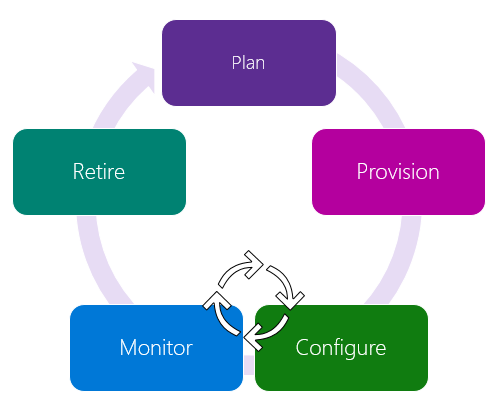
\includegraphics[scale=0.5]{images/hubdevmgmt-azure.png}
\caption{IoT Management Azure \cite{IoTMgmtAzure}}
\end{figure}
\subsubsection{Plan}
In der Planungsphase möchte man aufgrund von vorliegenden Daten eine Veränderung am System vornehmen. Um fundierte Entscheide in der Planungsphase zu ermöglichen werden Daten und Messwerte von Devices benötigt. Je einfacher diese Daten zugänglich-, respektive abfragbar sind, desto qualitativ hochwertiger und exakter kann geplant werden.
\subsubsection{Provision}
Neue Geräte müssen vor der produktiven Nutzung bereitgestellt werden. Dieser Prozess kann mehrere Personen und Aufgaben involvieren. Grundsätzlich werden neue Geräte in ein bestehendes System eingebunden oder ein komplett neues System aufgebaut.
\subsubsection{Configure}
Damit ein Device in den vorgesehenen Zustand versetzt werden kann benötigt es eine Konfiguration. Bei einer grossen Anzahl Devices empfiehlt es sich diesen Prozess bestmöglichst zu automatisieren. Dazu müssen alle Beteiligten  
\subsubsection{Monitor}
In der Monitoringphase sollen die Zustände der Devices überwacht werden. Ziel ist es, die Funktionalität und Korrektheit des angestrebten Verhalten sicherzustellen. Dies wird mittels periodischer Abfragen oder Observations sichergestellt. 
\subsubsection{Retire}
Am Ende des Lebenszyklus sollen Geräte geordnet aus dem System entfernt werden. Dabei gilt es den Prozess bestmöglich zu automatisieren und allfällige Vorschriften betreffend Datensicherheit und Datenschutz zu beachten. Andere Systeme wie das Inventar könnten ebenfalls in diesem Prozess beteiligt sein.
\section{Device Management Aufgaben}

\subsection{Provisionierung und Authentisierung}
\subsection{Konfiguration}
\subsection{Monitoring und Diagnose}
\subsection{Maintenance und Update}
\subsection{Security Management}

\section{}




















